\section{Literature Review}

\begin{comment}
This section can be developed starting from what you have reviewed and discussed in your previous reports, adjusted according to the feedback and indications provided by your supervisor(s). This section needs to flow logically, and this does not always imply that the material is chronological. By the end, the reader should have a clear appreciation of what the major work in the field was, why it is relevant to the current project, and where the unknowns and questions lie (research gaps) – these are the issues that you are going to address with your thesis research.

\subsection{\textbf{You can use subtitles like this to organize content within sections}}

An indicative length for the literature-review section is \textbf{~15 pages} (try to be concise and report significant information, rather than all information). Remember to reference properly any material that you obtain from literature or other sources. If you are unsure how to discuss literature properly, find a really good review paper on your topic, or if there isn’t one, a similar topic, and you will have a good example to refer to.
\end{comment}

\subsection{Principles of Photovoltaic Modules}
To understand the reduction in efficiency experienced by photovoltaic modules at increased temperatures, it is first necessary to examine the fundamental principles underlying their operation.\par

% Photovoltaic Module Definition + % Photoelectric Effect
Photovoltaic modules, commonly known as solar panels, are devices that convert sunlight into electrical energy \cite{EnelGreenPower2025PhotovoltaicModule, USDEPARTMENTofENERGY2024}. Sunlight is made up of massless particles called photons, which possess a certain amount of energy. When these photons strike the surface, they knock electrons off of it, known as photoelectrons. This is known as the photoelectric effect, shown in Figure \ref{fig:photoelectric_effect_diagram}.

\begin{wrapfigure}{r}{0.4\textwidth}
    \vspace{-2.5em}
    \centering
    \includegraphics[width=0.4\textwidth]{Figures/photoelectric_effect_diagram.png}
    \caption{Photoelectric Effect Diagram \cite{KhanAcademy2025PhotoelectricEffect}.}
    \label{fig:photoelectric_effect_diagram}
\end{wrapfigure}

The photoelectric effect will only occur if the frequency of the radiation is greater than the threshold frequency of the metal. The threshold frequency is the minimum frequency of light that causes electrons to be emitted from a material. The proportional relationship that exists between the threshold frequency, $f_0$, and the work function, $\phi_0$, is shown in Equation \ref{eq:work_function}.
\begin{equation}
    h_pf_0 = \phi_0+\text{K.E.}
    \label{eq:work_function}
\end{equation}
The work function refers to the minimum amount of energy needed to remove an electron from a metal surface. If photons with enough energy hit the surface, they can transfer their energy to the electrons allowing them to escape. If the energy of the incident photons is less than the work function, no electrons will be emitted, regardless of light intensity \cite{ScienceABC2023}.\par

% An Explanation of How Photovoltaic Modules Work
A photovoltaic module is made up of multiple photovoltaic cells, commonly known as solar cells. Each photovoltaic cell is made of semiconductor material, which is placed between the conductive layers. The most common semiconductor material used to make photovoltaic cells is silicon, accounting for 95\% of photovoltaic modules sold worldwide \cite{USDEPARTMENTofENERGY2024CellBasics}. These photovoltaic cells use the photovoltaic effect to convert solar energy into electrical energy.
\begin{figure}[H]
    \centering
    \vspace{-0.5em}
    \includegraphics[width=0.7\textwidth]
    {Figures/photovoltaic_cell_diagram.jpg}
    \vspace{-0.5em}
    \caption{Photovoltaic Cell Structure Diagram \cite{Gupta2020}.}
    \label{fig:photovoltaic_cell_diagram}
\end{figure}
\vspace{-1.5em}

As shown in Figure \ref{fig:photovoltaic_cell_diagram}, a silicon photovoltaic cell is composed of two different layers of silicon: an n-type silicon layer, which has additional electrons, and a p-type silicon layer, which has extra spaces for electrons, called holes.\par

Both the n-type and p-type silicon layers undergo a process known as doping; whereby specific impurities are intentionally introduced into an intrinsic semiconductor to enhance its electrical conductivity. The n- type silicon layer is doped with atoms such as arsenic or phosphorus, which possess one more valence electron than silicon atoms, thereby introducing additional free electrons into the material. Consequently, the n-type layer becomes negatively charged. Conversely, the p-type silicon layer is doped with elements such as boron or gallium, which possess one fewer valence electron than silicon atoms, creating electron deficiencies known as holes. As a result, the p-type layer acquires a positive charge. At the interface between the n-type and p-type layers, surplus electrons from the n-type region migrate to fill the holes in the p-type region, establishing an electric field across the p–n junction. This region is referred to as the depletion zone \cite{CircuitBread2019}.\par

When a photon strikes the silicon photovoltaic cell with the required energy, an electron is knocked out of its bond. Because of the electric field at the p-n junction, the negatively charged electron moves toward the n-side, while the resulting positively charged hole is attracted to the p-side. The free electrons are collected by thin metal fingers positioned at the top of the photovoltaic cell, before travelling through an external circuit. After electrical work is performed, the electrons are returned to the conductive aluminium sheet positioned at the back of the photovoltaic cell. Since electrons follow a continuous cycle and are the only moving components, there is no wear and tear, allowing photovoltaic cells to last for decades. \cite{TED-Ed2016} However, despite the absence of mechanical degradation, photovoltaic cells exhibit performance limitations under certain operating conditions.

\subsection{Performance Limitations of Photovoltaic Modules}
A major limitation of photovoltaic modules is their declining electrical efficiency, particularly at high temperatures. A review led by S. Dubey of Nanyang Technological University found that standard photovoltaic modules typically convert 6-20\% of incoming solar radiation into electrical energy. The remaining 80-94\% is mostly converted into heat, increasing the module’s temperature and further lowering its efficiency \cite{Dubey2013}.\par

% An active cooling system for photovoltaic modules - H.G. Teo
\begin{wrapfigure}{r}{0.65\textwidth}
    \vspace{-1.85em}
    \centering
    \includegraphics[width=0.65\textwidth]{Figures/electrical_efficiency_vs_temperature_pv_module.png}
    \vspace{-2em}
    \caption{Electrical efficiency as a function of PV temperature \cite{Teo2012}.}
    \label{fig:electrical_efficiency_vs_temperature_pv_module}
    \vspace{-2em} % <-- pulls text up closer
\end{wrapfigure}

A 2010 study led by H.G. Teo from the National University of Singapore refined Dubey et al.'s electrical efficiency range to 8-14\%. In the study, Teo et al. focused on comparing the electrical efficiency of photovoltaic modules under cooling and non-cooling conditions. Teo et al. observed that the electrical efficiency of the photovoltaic module decreased as the temperature of the module increased, as shown in Figure \ref{fig:electrical_efficiency_vs_temperature_pv_module}.

This inverse linear relationship between the temperature and the electrical efficiency of a photovoltaic module is attributed to the band gap reduction, which occurs as the module's temperature increases. % An explanation as to how increased module temperature leads to band gap reduction
In 1931, A.H. Wilson's paper, \textit{The Theory of Electronic Semi-Conductors}, introduced the idea that semiconductors have a small but finite band gap that affects their electrical conductivity \cite{Il1931}. The band gap represents the amount of energy that an electron must possess to jump from the valence band, where valence electrons are confined, to the conduction band. When valence electrons receive enough energy from an external source, they are able to undergo this band transition, which allows the material to conduct electricity \cite{CircuitBread2018}. As the temperature of the photovoltaic module increases, the valence electrons in the semiconductor material are excited. Thus, the energy required for an electron to transition from the valence band to the conduction band decreases, indicated by a reduced band gap \cite{RenewableTek2025}.\par

% Electrical efficiency of a photovoltaic module
\subsubsection{The Effect of Band Gap Reduction on Photovoltaic Module Performance}
To understand the proportional relationship between the band gap and the electrical efficiency, an inspection of the formula used to calculate the electrical efficiency of a photovoltaic cell, shown in Equation \ref{eq:pv_cell_efficiency_function}, is required \cite{HonsbergSolarEfficiency}.
\begin{equation}
    \eta = \frac{V_\text{OC}I_\text{SC}FF}{P_\text{in}}
    \label{eq:pv_cell_efficiency_function}
\end{equation}
The open circuit voltage, $V_\text{OC}$, short circuit current, $I_\text{SC}$, and fill factor, $FF$, are all affected by the band gap. Therefore, an investigation into the effect of a reduced band gap on these aforementioned variables is necessary to evaluate the impact that the band gap has on the electrical efficiency of the photovoltaic module.\par

% Open circuit voltage
\textbf{Open Circuit Voltage Analysis}\par
A 1994 study led by P. Baruch from the University of Paris derived a formula for determining the minimum value of the diode saturation current, as shown in Equation \ref{eq:minimum_diode_saturation_current}.
\begin{equation}
    J_0 = \frac{q}{k_b} \frac{15\sigma}{\pi^4} T^3 \int_{z}^{\infty} \frac{x^2}{e^x - 1}\,dx
    \label{eq:minimum_diode_saturation_current}
\end{equation}
where $z = \frac{E_G}{k_bT}$ \cite{Baruch1995}. A casual inspection of Equation \ref{eq:minimum_diode_saturation_current} reveals a relationship between the band gap energy, $E_g$, and the diode saturation current, $J_0$. However, it is not immediately obvious what the nature of the relationship is due to the complexity of the integral function.\par

\begin{figure}[h]
    \centering
    \begin{minipage}{0.495\textwidth}
        \centering
        \includegraphics[width=\textwidth]{Figures/diode_saturation_current_bandgap_graph.png}
        \caption{Diode saturation current as a function of band gap \cite{HonsbergOpen-CircuitVoltage}.}
        \label{fig:diode_saturation_current_bandgap_graph}
    \end{minipage}
    \hfill
    \begin{minipage}{0.465\textwidth}
        \vspace{-0.1em}
        \centering
        \includegraphics[width=\textwidth]{Figures/open-circuit_voltage_bandgap_graph.png}
        \caption{$V_\text{OC}$ as a function of band gap for a cell with AM 0 and AM 1.5 \cite{HonsbergOpen-CircuitVoltage}.}
        \label{fig:open-circuit_voltage_bandgap_graph}
    \end{minipage}
\end{figure}

Just over a decade later, Michael Y. Levy and Christiana Honsberg from the University of Delaware proposed a method to evaluate the integral in Baruch's formula \cite{Levy2006RapidApplications}. Then, in 2017, Honsberg worked with Stuart Bowden to graph the relationship between the diode saturation current and the band gap based on this method, as shown in Figure \ref{fig:diode_saturation_current_bandgap_graph}. Honsberg and Bowden used the diode saturation current values, $J_0$, from Figure \ref{fig:diode_saturation_current_bandgap_graph}, denoted as $I_0$ in Equation \ref{eq:open_circuit_voltage_function}, to calculate the open-circuit voltage, $V_\text{OC}$, as a function of the band gap. The linear proportional relationship between the band gap and the open-circuit voltage is shown in Figure \ref{fig:open-circuit_voltage_bandgap_graph}. Thus, the reduced band gap due to the increased temperature of the photovoltaic module leads to a decrease in the open-circuit voltage \cite{HonsbergOpen-CircuitVoltage}.
\begin{equation}
    V_{OC} = \frac{\zeta k_b T}{q} \times \ln\left(\frac{I_L}{I_0} + 1\right)
    \label{eq:open_circuit_voltage_function}
\end{equation}

% Short circuit current
\textbf{Short Circuit Current Analysis}\par
\begin{wrapfigure}{r}{0.5\textwidth}
    \vspace{-5.75em}
    \centering
    \includegraphics[width=\linewidth]{Figures/short_circuit_current_density_bandgap_graph.png}
    \caption{$J_\text{SC}$ as a function of band gap for a cell with AM 0 and AM 1.5. \cite{HonsbergShort-CircuitCurrent}}
    \label{fig:short_circuit_current_density_bandgap_graph}
\end{wrapfigure}

Honsberg and Bowden also graphed the relationship between the band gap and the short circuit current density, as shown in Figure \ref{fig:short_circuit_current_density_bandgap_graph}. From Figure \ref{fig:short_circuit_current_density_bandgap_graph}, it is evident that a band gap reduction corresponds to an increase in the short circuit current density. Equation \ref{short_circuit_current_function} shows a linearly proportional relationship between the short circuit current and the short circuit current density.
\begin{equation}
    I_\text{SC} = J_\text{SC}A
    \label{short_circuit_current_function}
\end{equation}
Therefore, a decrease in the band gap leads to an increase in the short-circuit current \cite{HonsbergShort-CircuitCurrent}.\par

% Fill Factor
\textbf{Fill Factor Analysis}\par
In 1981, M.A. Green of the University of New South Wales proposed an empirical expression for the fill factor, as shown in Equation \ref{eq:fill_factor_function}.
\begin{equation}
    FF = \frac{v_\text{OC} - \ln\ (v_\text{OC} + 0.72)}{v_\text{OC} + 1}
    \label{eq:fill_factor_function}
    \vspace{0.75em}
\end{equation}
where $v_\text{OC}$ is defined as a normalised $V_\text{OC}$: $v_\text{OC} = \frac{q}{nk_bT} V_\text{OC}$ \cite{Green1981}. As established earlier in Figure \ref{fig:open-circuit_voltage_bandgap_graph}, a band gap reduction corresponds to a decrease in the open-circuit voltage. An inspection of Equation \ref{eq:fill_factor_function} reveals that a decline in the open-circuit voltage and an increase in the temperature of the photovoltaic module causes a decrease in the fill factor. Therefore, it can be concluded that a band gap reduction causes a decrease in the fill factor.\par

% Resultant conclusion
To summarise, the band gap reduction that arises due to the increased temperature of the photovoltaic module causes a decrease in the open-circuit voltage, an increase in the short circuit current and a decrease in the fill factor. While the short circuit current does increase, it is ultimately outweighed by the decrease in the open-circuit voltage and fill factor, leading to a decrease in the module's electrical efficiency.

% Additional factors
\subsubsection{Environmental and Operational Factors Limiting Photovoltaic Module Performance}
In addition to temperature, other environmental factors like shade and air pollution limit the electrical efficiency of photovoltaic modules. A 2013 study led by A. Dolara from the Polytechnic University of Milan found that shade significantly affects the performance of photovoltaic modules. Dolara et al. observed a 31\% drop in the power generated by a single photovoltaic cell when 50\% of the cell was subjected to shade \cite{Dolara2013}. In 2001, E. Asl-Soleimani et al. from the University of Tehran concluded that air pollution also reduced the energy output of photovoltaic modules by up to 60\% \cite{Asl-Soleimani2001}. Furthermore, operational factors like poor module maintenance can lead to dust buildup, significantly reducing power generation. A review led by K. Hasan in 2021 stated a 60-70\% reduction in power generation due to the deposition of dust in humid conditions \cite{Hasan2022}. Although shade, air pollution, and dust accumulation influence photovoltaic module performance, this thesis focuses on temperature due to its unavoidable impact on module efficiency. In contrast to other environmental and operational factors that are site-specific or mitigable through maintenance, temperature rise is inherently linked to solar irradiation, the fundamental source of photovoltaic energy.

% Link the heat transfer paragraphs to the limitations paragraphs
In 1961, William Shockley and Hans Queisser published their paper, \textit{Detailed Balance Limit of Efficiency of p-n Junction Solar Cells}, in which they established the theoretical maximum efficiency of silicon-based solar cells to be approximately 30\% under standard illumination conditions \cite{Shockley1961}. In the real world however, photovoltaic cells are prevented from reaching this limit due to the factors previously discussed. Thus, due to the important role that photovoltaic modules play in the future of global energy, methods to reduce the impact that these factors have on the performance of photovoltaic modules are constantly being investigated.\par

In conjunction with establishing an inverse linear relationship between temperature and the electrical efficiency of photovoltaic modules, Teo et al. also observed that, under identical meteorological conditions, modules without active cooling operated at significantly higher temperatures than those with active cooling. Consequently, Teo et al.'s implementation of active cooling improved module efficiency from 8–9\% to 12–14\%, shown in Figure \ref{fig:electrical_efficiency_vs_temperature_pv_module} \cite{Teo2012}. As a result, to mitigate the reduction in electrical efficiency caused by increased photovoltaic module temperature, heat transfer-based cooling methods are investigated and employed worldwide.

\subsection{Heat Transfer in Photovoltaic Modules}
The fundamental concept of heat transfer is the process by which heat energy moves from one system or body to another as a result of a temperature difference. This transfer of heat can occur via conduction, convection or radiation. Figure \ref{fig:fundamental_concept_of_heat_transfer_diagram} demonstrates the fundamental concept of heat transfer in the context of a photovoltaic module.\par

\begin{figure}[H]
    \centering
    \includegraphics[width=1\textwidth]{Figures/fundamental_concept_of_heat_transfer_diagram.pdf}
    \vspace{-1.5em}
    \caption{Fundamental concept of heat transfer on a photovoltaic module. Adapted from \cite{HonsbergHeatModules}.}
    \label{fig:fundamental_concept_of_heat_transfer_diagram}
\end{figure}
\vspace{-1.5em}

In Figure \ref{fig:fundamental_concept_of_heat_transfer_diagram}, conductive heat transfer through the layers of the photovoltaic module and the mounting are observed. Additionally, heat is transferred from the surface of the photovoltaic module to the surrounding air via convection. Finally, the module emits thermal radiation to its surroundings, contributing to radiative heat transfer. In 2020, P. Dwivedi from the Maulana Azad National Institute of Technology, Bhopal, analysed the percentage distribution of heat loss across the different modes of heat transfer, shown in Table \ref{tab:heat_loss_from_pv_module} \cite{Dwivedi2020}.

\renewcommand{\arraystretch}{1.5} % increase vertical spacing
\begin{table}[h]
    \centering
    \caption{Heat loss from photovoltaic module \cite{Dwivedi2020}.}
    \begin{tabularx}{\textwidth}{l >{\hspace{4cm}}X l} % add horizontal space to middle column
        \toprule
        \textbf{S. No} & \textbf{Heat loss from module} & \textbf{Percentage (\%)} \\
        \midrule
        1 & Conduction through mounting & 2 \\
        2 & Convection from top surface & 42 \\
        3 & Convection from bottom surface & 24 \\
        4 & Radiation from top surface & 21 \\
        5 & Radiation from bottom surface & 11 \\
        \bottomrule
    \end{tabularx}
    \label{tab:heat_loss_from_pv_module}
\end{table}
\renewcommand{\arraystretch}{1} % reset back to default

An inspection of Table \ref{tab:heat_loss_from_pv_module} reveals that convection is the dominant mode of heat transfer in photovoltaic modules. Consequently, a given percentage increase in the rate of convective heat transfer will have a greater impact on overall module heat dissipation than an equivalent increase in conductive or radiative heat transfer. Therefore, the following subsections will examine the effectiveness of conduction-, convection-, and radiation-based cooling methods in reducing photovoltaic module temperatures to enhance overall efficiency, with particular emphasis on convection-based approaches.

\subsubsection{Conduction}
Conduction is the transfer of energy from the more energetic particles of a substance to the adjacent less energetic ones because of interactions between the particles. The formula commonly used to calculate the rate of heat conduction is shown in Equation 7 \cite{engel2014IntroductionAndBasicConcepts}.
\begin{equation}
    \dot{Q}_\text{cond}=-kA\frac{\Delta T}{\Delta x}
\end{equation}

Several conduction-based cooling methods have been widely adopted, with heat sinks and phase change materials (PCMs) being among the most prominent. A heat sink is a component used in thermal management strategies to transfer heat effectively. Its design is optimised to dissipate heat \cite{Kumar2024}. The use of a heat sink increases the cross-sectional area that the heat is being transferred to, denoted as $A$ in Equation 7. Through further inspection of Equation 7, it is observed that the increased cross-sectional area, $A$, results in an increased rate of conductive heat transfer, $\dot{Q}_\text{cond}$. A study led by S.N. Razali from the National University of Malaysia investigated the effect of
multidirectional tapered fin heat sinks (MTFHS) on photovoltaic modules. Razali et al. found that the proposed MTFHS reduced the module’s temperature by 12 \textdegree C, indicating enhanced conductive heat transfer, which consequently improved the photovoltaic module’s efficiency by 1.53\% \cite{Razali2023}.\par

A phase change material is a material that can change its state from solid to liquid and vice versa by releasing and storing thermal energy \cite{Nicholas2019}. When the surrounding temperature rises above the PCM’s melting point, it liquefies, drawing heat away from the photovoltaic module. Conversely, when the temperature drops below the melting point, the PCM solidifies, releasing the stored heat back into the environment. A 2023 study by B. Hussain and colleagues at the Capital University of Science \& Technology found that incorporating PCM lowered the surface temperature of photovoltaic modules by 13.1 \textdegree C, resulting in a 6.85\% increase in efficiency \cite{Hussain2023}.

\subsubsection{Radiation}
Radiation is the energy emitted by matter in the form of electromagnetic waves (or photons) due to changes in the electronic configurations of the atoms or molecules. In the context of heat transfer, the focus is on thermal radiation, which is the energy emitted by bodies due to their temperature. The formula 
commonly used to calculate the rate of radiative heat transfer is shown in Equation 8 \cite{engel2014IntroductionAndBasicConcepts}.
\begin{equation}
    \dot{Q}_\text{rad} = \varepsilon \sigma A_s (T_s^4-T_{surr}^4)
\end{equation}
In 2018, a study led by B. Zhao from the University of Science and Technology of China investigated the performance impact of radiation-based cooling methods on photovoltaic modules. Zhao et al. modified a photovoltaic module by adding a polydimethylsiloxane (PDMS) film on its top surface. PDMS is known to have high emissivity in the mid-infrared range (8-13) micrometres \cite{Song2020}. Through an inspection of Equation 8, it is observed that an increased emissivity, $\varepsilon$, causes an increase in the rate of radiative heat transfer, $\dot{Q}_\text{rad}$. In theory, the increased radiative heat transfer of the photovoltaic module lowers the module’s temperature and improves its efficiency. However, Zhao et al. found that the temperature of the photovoltaic module was only reduced by 1.75 K in the ideal case. Furthermore, this result was achieved using a simulated environment. Thus, Zhao’s team concluded that enhanced radiative cooling offers limited practical benefit for photovoltaic module temperature reduction \cite{Zhao2018}.

\subsubsection{Convection}
Convection is the mode of energy transfer between a solid surface and the adjacent liquid or gas that is in motion. The formula commonly used to calculate the rate of convective heat transfer can be expressed by Newton’s law of cooling, shown in Equation 9 \cite{engel2014IntroductionAndBasicConcepts}.
\begin{equation}
    \dot{Q}_\text{conv} = hA(T_s-T_\infty)
\end{equation}
Convection is not a fundamental heat transfer mechanism; rather, it is a combined phenomenon, where heat conduction occurs in the presence of fluid motion. Convection can be broadly categorised into two types: natural convection, also referred to as free convection, and forced convection \cite{engel2014FundamentalsOfConvection}.

\textbf{Natural Convection \& Relevant Cooling Methods}\par
\begin{wrapfigure}{r}{0.4\textwidth}
    \centering
    \vspace{-4.5em}
    \includegraphics[width=0.9\linewidth, trim=0 0 0 15, clip]{Figures/cooling_of_boiled_egg_natural_convection.pdf}
    \vspace{-1.5em}
    \caption{The cooling of a boiled egg from natural convection  
    \cite{engel2014IntroductionAndBasicConcepts}.}
    \label{fig:natural_convection_egg}
    \vspace{-2em}
\end{wrapfigure}

Natural convection is the process by which heat transferred to a fluid raises its temperature, reducing its density and generating buoyant forces. These forces cause the warmer, lighter fluid to rise, carrying the absorbed heat to 
another location where it can be dissipated \cite{Zohuri2020}. Figure \ref{fig:natural_convection_egg} illustrates natural convective heat transfer in the context of cooling a hot egg.

\textit{Tilt Angle Optimisation}\par
The tilt angle of a photovoltaic module significantly influences natural convective heat transfer, as it alters the buoyancy-driven airflow around the module’s surface. A 2021 study led by A. Abdulmunem from the University of Malaya, Malaysia, investigated the impact of tilt angle on the performance of photovoltaic systems. Abdulmunem et al. observed that as the tilt angle increased from 0\textdegree  (horizontal) to 90\textdegree (vertical), the temperature reduction in the photovoltaic cell increased from -0.4\% to -12\%. This trend was attributed to enhanced natural convective heat transfer which acts to improve photovoltaic module efficiency. Consequently, Abdulmunem et al. concluded that 
increasing the tilt angle of the photovoltaic module away from the horizontal axis and towards the vertical axis improves the rate of convective heat transfer \cite{Abdulmunem2021}.

\textit{Natural Convection Boundary Layers}\par
To understand the effect of the tilt angle on natural convective heat transfer, it is necessary to first understand the velocity and thermal boundary layers. The velocity boundary layer describes how the fluid’s motion adjusts from being stationary at the surface to moving freely away, while the thermal boundary layer describes how heat diffuses into or from the fluid at the surface. The thermal and velocity boundary layers are interconnected, with fluid motion influencing heat transfer, and their relative thickness depends on the fluid’s properties. The relationship between the thermal and velocity boundary layers is characterised by the Prandtl number, Pr.\par

As shown in Figure \ref{fig:horizontal_plate_nc}, at lower tilt angles (near horizontal), the heated air tends to remain attached to the surface for a longer duration, as the buoyancy forces are predominantly vertical. This results in the formation of a thicker and more stable thermal boundary layer, which promotes relatively weak convection. In contrast, as shown in Figure \ref{fig:inclined_plate_nc}, when the surface aligns more closely with the direction of the buoyant forces, the hot air can rise more freely along the surface. This facilitates a thinner thermal boundary layer and an increased air velocity near the surface, thereby enhancing convective heat transfer.

\begin{figure}[h]
    \centering
    \vspace{1em}
    \begin{minipage}{0.48\linewidth}
        \centering
        \includegraphics[width=0.66\linewidth]{Figures/horizontal_plate_nc.jpg}
        \caption{Natural convective heat transfer on a horizontal plate. Adapted from \cite{engel2014NaturalConvection}.}
        \label{fig:horizontal_plate_nc}
    \end{minipage}
    \hfill
    \begin{minipage}{0.48\linewidth}
        \centering
        \includegraphics[width=0.8\linewidth]{Figures/inclined_plate_nc.jpg}
        \caption{Natural convective heat transfer on a inclined plate. Adapted from \cite{engel2014NaturalConvection}.}
        \label{fig:inclined_plate_nc}
    \end{minipage}
\end{figure}

\textit{Tilt Angle Optimisation: A Theoretical Confirmation}\par
Abdulmunem’s conclusion is also in excellent agreement with the theoretical relationship between the photovoltaic module’s tilt angle and the natural convective heat transfer rate. The Rayleigh number, $\mathrm{Ra_L}$, which can be calculated using Equation 10, is the ratio of buoyancy forces and (the products of) thermal and momentum diffusivities \cite{engel2014NaturalConvection}.
\begin{equation}
    \mathrm{Ra_L} = \frac{g\beta(T_s-T_\infty)L_c^3}{\nu \alpha}
\end{equation}
For an inclined photovoltaic module between 0\textdegree and 60\textdegree, the gravitational force, $\mathrm{Ra_\theta}$, is replaced with $g\,sin(\theta)$, where $\theta$ represents the tilt angle between the horizontal axis and the photovoltaic module, shown in Figure 11.

\begin{wrapfigure}{r}{0.3\textwidth}  % 'r' = right, width = 40% of text width
    \vspace{-0.75em}
    \centering
    \includegraphics[width=\linewidth, trim=0 0 0 20, clip]{Figures/inclined_plate.pdf} 
    % trim=left bottom right top; top cropped by 50 units
    \vspace{-5.8em}
    \caption{Inclined photovoltaic module. Adapted from \cite{engel2014NaturalConvection}.}
    \label{fig:inclined_plate}
    \vspace{-1em}
\end{wrapfigure}

Thus, Equation 11 is the appropriate mathematical expression for the Rayleigh number of a tilted photovoltaic module, $\mathrm{Ra_\theta}$, \cite{engel2014NaturalConvection}.
\begin{equation}
    \mathrm{Ra_\theta} = \frac{g\, \sin(\theta)\, \beta\ (T_s-T_\infty)L_c^3}{\nu \alpha}
\end{equation}
A casual inspection of Equation 11 indicates that the Rayleigh number for a tilted photovoltaic module, $\mathrm{Ra_\theta}$, is directly proportional to the tilt angle, $\theta$, within the range of 0\textdegree to 60\textdegree\, \cite{engel2014NaturalConvection}. Therefore, increasing the tilt angle within this range results in a corresponding increase in the Rayleigh number.\par

The Nusselt number, Nu, is the ratio of convective to conductive heat transfer \cite{Basu2019}. For simple empirical correlations in natural convection, an exponential relationship exists between the average Nusselt number, Nu, and the relevant Rayleigh number, shown in Equation 12. \cite{engel2014NaturalConvection}
\begin{equation}
    \mathrm{Nu} = C\,\mathrm{Ra_\theta^\gamma}
\end{equation}
Therefore, the increase in the Rayleigh number leads to an increase in the Nusselt number. Moreover, Equation 13 reveals that an increase in the Nusselt number, Nu, causes an increase in the convective heat transfer coefficient, $h$, \cite{engel2014NaturalConvection}.
\begin{equation}
    h = \frac{\mathrm{Nu}\times k}{L_c}
\end{equation}
Finally, an inspection of Equation 9 reveals that an increase in the convective heat transfer coefficient, $h$, results in a higher convective heat transfer rate, $\dot{Q}_\mathrm{conv}$, thereby supporting Abdulmunem et al.’s experimental findings \cite{engel2014IntroductionAndBasicConcepts}.\par

While a vertical photovoltaic module improves natural convective heat transfer, it limits the surface area that is directly exposed to the sun, reducing power output. Thus, a tilt angle of 45\textdegree$\ $from the horizontal axis (as in earlier NOCT testing \cite{InternationalElectrotechnicalCommission2005}) is generally used in photovoltaic module testing because it represents more realistic conditions.

\textit{Comparing Natural and Forced Convection Effects in Photovoltaic Module Temperature Reduction}\par
Natural convection-based cooling methods can effectively reduce an object’s temperature; however, in photovoltaic modules, forced convection is significantly more efficient at transferring heat to the surroundings, resulting in greater improvements in module efficiency. A 2021 study led by A. Almuwailhi from King Saud University investigated the impact of both natural and forced convection cooling methods on the efficiency of photovoltaic modules. To promote natural convective heat transfer, Almuwailhi’s team experimented with various channel air gaps. The most promising configuration featured an air gap height of 120 mm, which led to a 1.2\% increase in photovoltaic module efficiency. For forced convection, Almuwailhi’s team used airflow velocities of 2 m/s and 3 m/s. The results revealed a 3.8\% increase in efficiency with 2 m/s airflow, and a 4\% increase with 3 m/s airflow \cite{Almuwailhi2023}. As a result, the remainder of this literature review will be dedicated to a comprehensive examination of forced convection-based cooling methods.

\textbf{Forced Convection \& Relevant Cooling Methods}\par
\begin{wrapfigure}{r}{0.4\textwidth}
    \centering
    \vspace{-5.2em}
    \includegraphics[width=\linewidth, trim=0 0 0 5, clip]{Figures/cooling_of_boiled_egg_forced_convection.pdf}
    \vspace{-2em}
    \caption{The cooling of a boiled egg from natural convection  
    \cite{engel2014IntroductionAndBasicConcepts}.}
    \label{fig:forced_convection_egg}
    \vspace{-2em}
\end{wrapfigure}

Forced convection is a mode of heat transfer in which fluid flow over a surface is induced by external means such as a fan, pump, or wind, rather than resulting from natural buoyancy forces \cite{engel2014IntroductionAndBasicConcepts}. Figure \ref{fig:forced_convection_egg} illustrates how forced convective heat transfer can be applied to cool a hot egg. Like natural convection, forced convection involves the development of velocity and thermal boundary layers that control momentum and heat transfer in the vicinity of the surface. Since boundary layer behaviour under forced convection differs from that in natural convection, it is important to examine the mechanisms governing their formation.

\textit{Forced Convection Boundary Layers}\par
Figure \ref{fig:velocity_boundary_layer} illustrates the velocity profile caused by parallel fluid flow over a flat plate. To understand this velocity profile, the fluid is modelled as a series of adjacent layers stacked on top of one another. The fluid particles in the layer closest to a solid surface are  subject to the no-slip condition, which states that their velocity must match that of the boundary, resulting in zero relative motion between  the  fluid  and  the  surface. Since photovoltaic modules remain stationary during operation, the fluid layer in direct contact with the surface has a velocity, $u$ = 0.\par

\begin{wrapfigure}{r}{0.4\textwidth}
    \centering
    \vspace{-1.9em}
    \includegraphics[width=1\linewidth]{Figures/velocity_boundary_layer.pdf}
    \vspace{-1.4em}
    \caption{Velocity boundary layer over a flat plate. Adapted from \cite{engel2014FundamentalsOfConvection}.}
    \label{fig:velocity_boundary_layer}
\end{wrapfigure}

The stationary fluid layer adjacent to the surface exerts frictional resistance on the fluid layer above it, reducing its velocity through shear interaction between layers moving at different speeds. This process propagates through successive fluid layers, each experiencing a reduction in momentum due to shear from the layer beneath, resulting in a velocity profile that increases with distance from the surface, but at a decreasing rate. At the boundary layer thickness, $\delta$, the plate has negligible effect on the velocity of the fluid. Thus, $\delta$, is typically defined as the distance from the surface where $u$ = 0.99$V$. Therefore, the velocity boundary layer can be defined as the region of flow above the plate, bounded by $\delta$, where the effects of viscous shearing forces are significant \cite{engel2014FundamentalsOfConvection}.\par

Figure \ref{fig:thermal_boundary_layer} shows the temperature profile that results due to the flow of parallel fluid over a flat plate. Given the focus on reducing photovoltaic module temperature, it is appropriate to illustrate a thermal boundary layer diagram where the plate surface is at a higher temperature than the surrounding fluid. The fluid particles adjacent to the surface of the plate reach thermal equilibrium  with  the  plate, adopting a temperature, $T_s$. This fluid layer transfers energy to the layer directly above it, resulting in a temperature gradient where each successive layer has a slightly lower temperature than the previous one, with the rate of decrease diminishing progressively.\par
\begin{wrapfigure}{r}{0.4\textwidth}
    \centering
    \vspace{-1em}
    \includegraphics[width=1\linewidth]{Figures/thermal_boundary_layer.pdf}
    \vspace{-2.5em}
    \caption{Thermal boundary layer over a flat plate. Adapted from \cite{engel2014FundamentalsOfConvection}.}
    \label{fig:thermal_boundary_layer}
    \vspace{-2em}
\end{wrapfigure}
The boundary layer thickness, $\delta_t$, represents the perpendicular distance from the flat plate at which the influence of the plate’s temperature, $T_s$, on the fluid temperature, $T_\infty$, becomes negligible. Thus, the thickness of the thermal boundary layer at any location on the surface occurs when $T = T_s - 0.99(T_s - T_\infty)$. Therefore, the thermal boundary layer is defined as the flow region above the surface, bounded by $\delta_t$, where the temperature variation in the direction normal to the surface is significant \cite{engel2014FundamentalsOfConvection}.\par

A thicker thermal boundary layer results in a more  gradual temperature gradient at the surface, reducing the effectiveness of convective cooling. To overcome this limitation, forced convection techniques are employed to disrupt and thin the boundary layer, enhancing the temperature gradient at the surface. This increase in the gradient leads to a higher convective heat transfer rate, which lowers the operating temperature of the photovoltaic module and improves its efficiency. Accordingly, the following section examines convection-based cooling strategies that aim to reduce boundary layer thickness.\par

\textit{Air-Based Cooling Methods}\par
In 2024, a study led by I. Al-Masalha from Al-Balqa Applied University investigated the enhancement of photovoltaic module efficiency through various cooling techniques, including air fans, water sprinklers, and hybrid systems. One of the approaches involved directing airflow over the surface of the modules using air fans. This method resulted in a module temperature reduction ranging from 6\% to 26\%, as shown in Figure \ref{fig:air_cooling_temperature_graph}. Correspondingly, this temperature decrease led to an improvement in electrical efficiency between 0.44\% and 1.45\%, as illustrated in Figure \ref{fig:air_cooling_efficiency_graph} \cite{Al-Masalha2024}.

\begin{figure}[ht]
    \centering
    \begin{minipage}{0.45\linewidth}
        \centering
        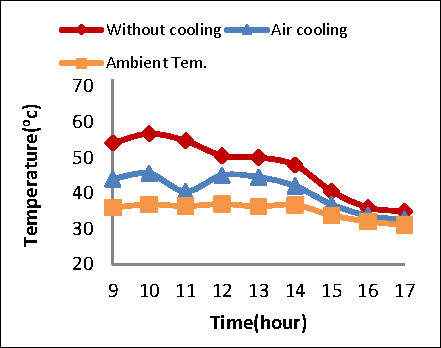
\includegraphics[width=\linewidth, trim=2 2 2 2, clip]{Figures/air_cooling_temperature_graph.pdf}
        \caption{Comparison of PV temperature when using air cooling over time \cite{Al-Masalha2024},}
        \label{fig:air_cooling_temperature_graph}
    \end{minipage}
    \hfill
    \begin{minipage}{0.45\linewidth}
        \centering
        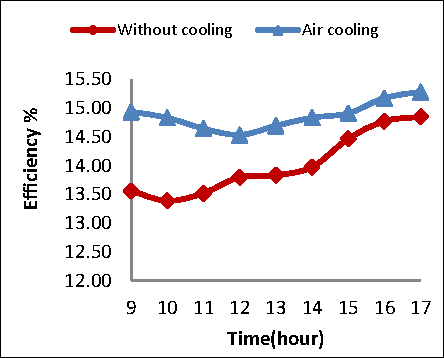
\includegraphics[width=\linewidth, trim=2 2 2 2, clip]{Figures/air_cooling_efficiency_graph.pdf}
        \caption{Comparison of efficiency when using air cooling over time \cite{Al-Masalha2024}.}
        \label{fig:air_cooling_efficiency_graph}
    \end{minipage}
\end{figure}

\textit{Water-Based Cooling Methods}\par
Al-Masalha et al.’s water cooling method involved spraying water directly onto the photovoltaic modules to dissipate heat. As illustrated in Figure \ref{fig:water_cooling_temperature_graph}, this technique resulted in a temperature reduction of the photovoltaic module ranging from 20.45\% to 35.44\%. Consequently, as shown in Figure \ref{fig:water_cooling_efficiency_graph}, this temperature reduction led to an efficiency improvement between 0.6\% and 1.8\% \cite{Al-Masalha2024}.

\begin{figure}[H]
    \centering
    \begin{minipage}{0.45\linewidth}
        \centering
        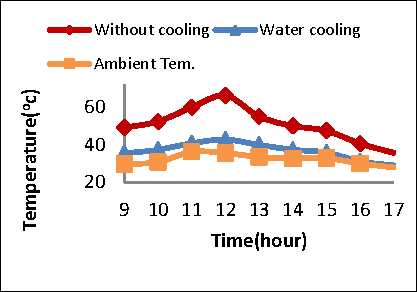
\includegraphics[width=\linewidth, trim=2 2 2 2, clip]{Figures/water_cooling_temperature_graph.pdf}
        \caption{Comparison of PV temperature when using water sprinklers over time \cite{Al-Masalha2024}.}
        \label{fig:water_cooling_temperature_graph}
        \vspace{-2em}
    \end{minipage}
    \hfill
    \begin{minipage}{0.45\linewidth}
        \centering
        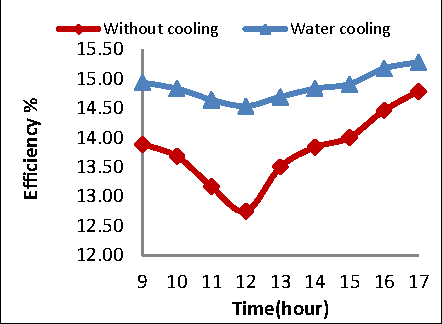
\includegraphics[width=\linewidth, trim=2 2 2 2, clip]{Figures/water_cooling_efficiency_graph.pdf}
        \caption{Comparison of efficiency when using water sprinklers over time \cite{Al-Masalha2024}.}
        \label{fig:water_cooling_efficiency_graph}
        \vspace{-2em}
    \end{minipage}
\end{figure}

\textit{Hybrid Cooling Methods}\par
In their final approach, Al-Masalha’s team developed a hybrid cooling system by combining water spraying and air-cooling techniques. This integrated method produced the most significant results in terms of both temperature reduction and efficiency improvement. The hybrid cooling system achieved a temperature reduction in the range of 30\% and 40\%, shown in Figure \ref{fig:hybrid_cooling_temperature_graph}. This substantial reduction in temperature led to an increase in photovoltaic module efficiency, ranging from 0.88\% to 2\%, as illustrated in Figure \ref{fig:hybrid_cooling_efficiency_graph} \cite{Al-Masalha2024}.\vspace{1em}

\begin{figure}[H]
    \centering
    \begin{minipage}{0.45\linewidth}
        \vspace{-1em}
        \centering
        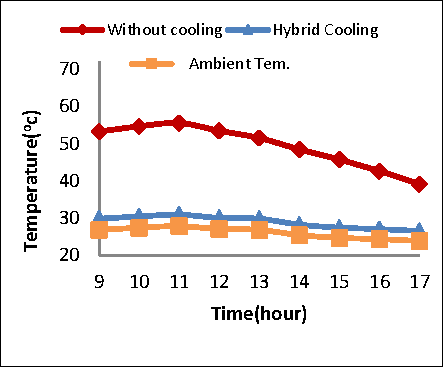
\includegraphics[width=\linewidth, trim=2 2 2 2, clip]{Figures/hybrid_cooling_temperature_graph.pdf}
        \vspace{-3.5em}
        \caption{Comparison of PV temperature when using hybrid cooling over time \cite{Al-Masalha2024}.}
        \label{fig:hybrid_cooling_temperature_graph}
    \end{minipage}
    \hfill
    \begin{minipage}{0.45\linewidth}
        \vspace{-0.5em}
        \centering
        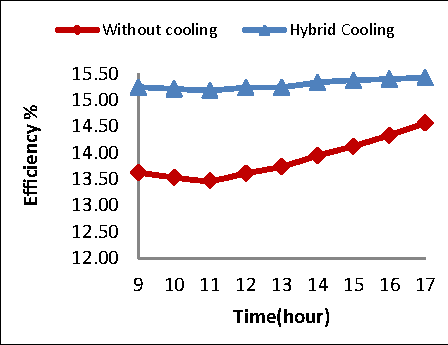
\includegraphics[width=\linewidth, trim=2 2 2 2, clip]{Figures/hybrid_cooling_efficiency_graph.pdf}
        \vspace{-2.5em}
        \caption{Comparison of efficiency when using hybrid cooling over time \cite{Al-Masalha2024}.}
        \label{fig:hybrid_cooling_efficiency_graph}
    \end{minipage}
\end{figure}\vspace{-1em}

\textit{Nano-fluid Based Cooling Methods}\par
In recent times, nanofluid-based cooling methods have emerged as a highly effective technique for enhancing the thermal management and overall efficiency of photovoltaic modules. In 2022, T.K. Murtadha et al. conducted an experimental investigation into the performance enhancement of photovoltaic modules using titanium dioxide nanofluids. Their findings indicated that higher nanoparticle concentrations correlated with improved heat dissipation, resulting in a maximum efficiency gain of 19.23\% under optimal nanofluid cooling conditions \cite{Murtadha2022}.

\textit{An Assessment and Conclusion on the Most Promising Cooling Method}\par
The studies conducted by Al-Masalha et al. \cite{Al-Masalha2024} and Murtadha et al. \cite{Murtadha2022} clearly demonstrate that water and nanofluid cooling methods outperform air-based cooling in terms of thermal regulation and efficiency improvement for photovoltaic modules. However, despite their superior performance, water and nanofluid cooling systems are significantly less prevalent than air cooling in photovoltaic applications. This disparity is primarily due to several practical limitations. Both water and nanofluid systems entail higher initial and operational costs, as well as increased system complexity \cite{Dwivedi2020, Suresh2018}. Additionally, they demand more frequent and intensive maintenance compared to air cooling systems, further escalating long-term expenses \cite{Samykano2023, Ponticorvo2022}. Moreover, the structural load associated with liquid- based cooling is greater due to the added weight of the coolant medium, which imposes additional design and material constraints \cite{Sakanova2016}. These factors collectively impact the cost-effectiveness of photovoltaic cooling strategies, rendering air cooling the most viable option for both commercial and residential implementations. Consequently, air cooling remains the most employed method for photovoltaic module thermal management \cite{Dwivedi2020}.\par

As was stated previously, Al-Masalha et al. implemented active cooling of photovoltaic modules using electric powered air fans to facilitate convective heat transfer \cite{Al-Masalha2024}. However, this approach incurs a parasitic energy cost, as external power is required to operate the fans. Vortex generators provide a passive cooling alternative that uses wind to induce localised turbulence and enhance convective heat transfer. Therefore, the following section explores the use of vortex generators to enhance the thermal management of photovoltaic modules.

\subsection{Vortex Generators}
Vortex generators are protrusions on a heat transfer surface that induce swirling flow around an axis, generating vortices that enhance convective heat transfer \cite{Awais2018}. Figure \ref{fig:vortex_generator} illustrates this phenomenon for a cylindrical vortex generator interacting with the surrounding fluid.
\vspace{-1em}
\begin{figure}[H]
    \centering
    \includegraphics[width=\linewidth]{Figures/vortex_generator.pdf}
    \vspace{-2em}
    \caption{Fluid flow over a cylinder. Adapted from \cite{VanTreuren2015}.}
    \label{fig:vortex_generator}
\end{figure}
\vspace{-1.5em}

Figure \ref{fig:vortex_generator} also draws attention to two key features associated with vortex generators: the forward stagnation point and the separation point. At the forward stagnation point, the fluid velocity, $u$, is zero, while the separation point marks the location where the airflow detaches from the surface of the object. At the separation point, vortices, referred to as Kármán vortices in the context of cylindrical bodies, are generated \cite{Wille1960}. These vortices promote mixing between the high-momentum outer fluid and the low-momentum near-wall fluid, enhancing momentum and energy exchange near the surface. This mixing thins the thermal boundary layer, thereby enhancing convective heat transfer as previously discussed. Section 2.4.1 presents the theoretical basis for the described flow behaviour.\par

\subsubsection{Vortex Generators: A Theoretical Confirmation}
The location of the separation point on a cylinder depends on the boundary layer’s transition from laminar to turbulent flow. This transition is primarily characterised by the Reynolds number, $\mathrm{Re}$, defined as the 
ratio of inertial to viscous forces in the fluid. For cylindrical shapes, the Reynolds number is found using Equation 14 \cite{engel2014ExternalForcedConvection}.
\begin{equation}
    \mathrm{Re_D} = \frac{\rho VD}{\mu} = \frac{VD}{\nu}
\end{equation}
The Reynolds number is closely related to the Nusselt number; however, for cylindrical vortex generators in cross flow, the relationship is not straightforward. To address this, Churchill and Bernstein (1977) proposed an empirical correlation to estimate the average Nusselt number for cross flow over a cylinder, $\mathrm{Nu_{cyl}}$, incorporating both the Reynolds and Prandtl numbers, as shown in Equation 15 \cite{engel2014ExternalForcedConvection}.
\begin{equation}
    \mathrm{Nu_{cyl}} = 0.3 + \frac{0.62 \mathrm{Re^{\frac{1}{2}}Pr^{\frac{1}{3}}}}{[1+(\frac{0.4}{\mathrm{Pr}})^{\frac{2}{3}}]^{\frac{1}{4}}}[1+(\frac{\mathrm{Re}}{282,000})^{\frac{5}{8}}]^{\frac{4}{5}}
\end{equation}
The average Nusselt number, $\mathrm{Nu_{cyl}}$, has a proportional relationship with the average convective heat transfer coefficient, $h$, shown in Equation 16 \cite{engel2014ExternalForcedConvection}.
\begin{equation}
    \mathrm{Nu_{cyl}} = \frac{hD}{k}
\end{equation}
Thus, the resulting convective heat transfer coefficient, $h$, can be used to determine the rate of convective heat transfer, as shown in Equation 9, thereby quantifying the effect of cylindrical vortex generators on heat transfer \cite{engel2014IntroductionAndBasicConcepts}.

\subsubsection{Vortex Generator-Based Cooling Methods}
A 2024 study led by Z. Zhou from the University of New South Wales investigated the effect of vortex 
generators on photovoltaic module cooling. Zhou et al. attached rectangular wing vortex generators, 
made from either aluminium sheet or 3D-printed thermally conductive polymer, to the rear side of the 
photovoltaic modules. Although the vortex generators were optimised for free convection, both designs 
successfully reduced the photovoltaic module temperature by 1.5 \textdegree C under low wind conditions and high irradiance. In scenarios with high module temperatures and windy conditions, the aluminium vortex generators achieved a greater cooling effect, reducing the module temperature by 2.5 \textdegree C \cite{ZiboZhou2024}. Zhou et al.’s observation of variations in results due to different vortex generator materials highlights the significant influence of vortex generator parameters on photovoltaic module cooling \cite{ZiboZhou2024}. As a result, several studies have investigated the influence of other vortex generator parameter modifications on the thermal performance of photovoltaic modules.

\textbf{Effect of Vortex Generator Orientation on Photovoltaic Module Temperature Reduction}\par
A 2023 study conducted by S. Schiffman from the University of New South Wales investigated the effect of vortex generator orientation on photovoltaic module temperature.
\begin{figure}[H]
    \centering
    \begin{minipage}{0.48\linewidth}
        \centering
        \includegraphics[width=\linewidth, trim=0 10 0 10, clip]{Figures/fwd_full_formation_page-0001.jpg}
        \vspace{-2em}
        \caption{Forward facing vortex generator arrangment. Adapted from \cite{Schiffmann2023}.}
        \label{fig:fwd_full_fomation}
    \end{minipage}
    \hfill
    \begin{minipage}{0.48\linewidth}
        \centering
        \includegraphics[width=\linewidth, trim=0 10 0 10, clip]{Figures/back_full_formation_page-0001.jpg}
        \vspace{-2em}
        \caption{Backward facing vortex generator arrangement. Adapted from \cite{Schiffmann2023}.}
        \label{fig:back_full_formation}
    \end{minipage}
    \vspace{-1em}
\end{figure}
Schiffman positioned 3D-printed vortex generators in two configurations: a forward-facing arrangement (Figure \ref{fig:fwd_full_fomation}) and a backward-facing arrangement (Figure \ref{fig:back_full_formation}). Schiffman's experiment revealed that although both configurations enhanced cooling of the photovoltaic module, the backward-facing arrangement consistently achieved greater temperature reductions across wind speeds of $1,\text{m/s}$, $2,\text{m/s}$, and $3,\text{m/s}$. Specifically, the backward-facing setup achieved mean temperature reductions of approximately $1.4\ ^\circ\text{C}$, $0.75\ ^\circ\text{C}$, and $0.7\ ^\circ\text{C}$, respectively \cite{Schiffmann2023}.

\textbf{Effect of Vortex Generator Shape on Photovoltaic Module Temperature Reduction}\par
Schiffman's results and experimental setup laid the foundation for further investigations into additional parameters influencing module cooling performance. Building on this work, I.R. Chaudhury examined the impact of vortex generator geometry on photovoltaic module cooling. Chaudhury tested several shapes, including cube, cylindrical, pyramid, inverted pyramid, and winglet configurations, shown in Figure \ref{fig:vortex_generator_shapes}. \par

\begin{wrapfigure}{r}{0.6\textwidth}
    \vspace{-2em}
    \centering
    \includegraphics[width=\linewidth, trim=0 0 0 0, clip]{Figures/vortex_generator_shapes.pdf}
    \vspace{-3em}
    \caption{VG Geometry Configurations. Adapted from \cite{Chaudhury2024}.}
    \label{fig:vortex_generator_shapes}
    \vspace{-2em}
\end{wrapfigure}

While winglet-shaped vortex generators reduced photovoltaic module temperature by $5\ ^\circ \text{C}$ at $1$ m/s, their free-convection based design meant that cooling effectiveness diminished at higher wind velocities. In contrast, cylindrical-shaped vortex generators demonstrated the most favourable trend, causing greater temperature reductions as the velocity increased. Thus, Chaudhury encouraged the selection of the cylindrical vortex generator for further experimentation, focusing on spacing configurations to promote turbulent flow in the stream-wise direction \cite{Chaudhury2024}.

\textbf{Effect of Vortex Generator Spacing on Photovoltaic Module Temperature Reduction}\par
\begin{wrapfigure}{r}{0.4\textwidth}
    \vspace{-2em}
    \centering
    \includegraphics[width=1\linewidth, trim=0 0 0 20, clip]{Figures/spacing_diagram.pdf}
    \vspace{-4em}
    \caption{Spacing direction of vortex generator array relative to the direction of airflow. Adapted from \cite{Zhou2024}.}
    \label{fig:spacing_diagram}
    \vspace{-4em}
\end{wrapfigure}

Consequently, in 2024, Z. Zhou investigated the effects of span-wise, $d_x$, and stream-wise, $d_y$, spacing of cylindrical vortex generators on photovoltaic module temperature reduction. The spacing direction of the vortex generator array relative to the direction of airflow is shown in Figure \ref{fig:spacing_diagram}.\par

For the span-wise spacing group, Zhou tested five values of horizontal spacing, $d_x$ ($26$ mm, $51$ mm, $102$ mm, $153$ mm, and $204$ mm), while maintaining a constant stream-wise spacing, $d_y$, of $79$ mm. Each configuration was subjected to forced convection wind speeds of $1.3$ m/s, $2.3$ m/s, and $3.3$ m/s.\par

Similarly, for the stream-wise spacing group, Zhou tested five values of vertical spacing, $d_y$ ($40$ mm, $79$ mm, $119$ mm, $158$ mm, and $198$ mm), with the span-wise spacing, $d_x$, fixed at $51$ mm. These configurations were subjected to forced convection wind speeds of $1$ m/s, $2$ m/s, and $3$ m/s.\par

The results indicated that $51$ mm span-wise spacing under a wind speed of $3.3$ m/s produced the greatest temperature reduction among the span-wise configurations, achieving a decrease of $2.15\ ^\circ\text{C}$. In the stream-wise group, a spacing of $79$ mm under a wind speed of $3$ m/s yielded the largest reduction, with a decrease of $2.51\ ^\circ\text{C}$ \cite{Zhou2024}.

\textbf{Effect of Vortex Generator Height on Heat Transfer}\par
\begin{wrapfigure}{r}{0.4\linewidth}
    \vspace{-2.1em}
    \centering
    \includegraphics[width=\linewidth]{Figures/huang_vg.png}
    \caption{Huang et. al's experimental setup diagram \cite{huang2023downstream}.}
    \label{fig:huang_vg}
    \vspace{-2em}
\end{wrapfigure}
In 2023, Y.X. Huang from National Cheng Kung University led a study investigating the downstream effects of turbulent flow past vortex generators. As illustrated in Figure \ref{fig:huang_vg}, the experimental setup employed rectangular-prism-shaped vortex generators, which were exposed to a constant wind speed, $M$, representing the Mach number.\par

Huang et al. employed pressure-sensitive paint to map the global surface patterns of flow over a flat plate in the presence of vortex generators. These patterns were examined at three different heights, defined as the ratio of the vortex generator height to the incoming boundary layer thickness: $h^* =\,$ 0.2, 0.5, and 1.0. As shown in Figure \ref{fig:huang_results_a}, Figure \ref{fig:huang_results_b}, and Figure \ref{fig:huang_results_c}, the downstream influence of the flow increased with the vortex generator height at a constant Mach number of $M = 0.83$ \cite{huang2023downstream}.\par

\begin{figure}[H]
    \centering
    \includegraphics[width=0.9\linewidth]{Figures/huang_results_a.png}
    \caption{Global surface pressure pattern for counter-rotating vane vortex generators at $M = 0.83$, $h^* = 1.0$ \cite{huang2023downstream}.}
    \label{fig:huang_results_a}
\end{figure}

\begin{figure}[H]
    \centering
    \includegraphics[width=0.9\linewidth]{Figures/huang_results_b.png}
    \caption{Global surface pressure pattern for counter-rotating vane vortex generators at $M = 0.83$, $h^* = 0.5$ \cite{huang2023downstream}.}
    \label{fig:huang_results_b}
\end{figure}

\begin{figure}[H]
    \centering
    \includegraphics[width=0.9\linewidth]{Figures/huang_results_c.png}
    \caption{Global surface pressure pattern for counter-rotating vane vortex generators at $M = 0.83$, $h^* = 0.2$ \cite{huang2023downstream}.}
    \label{fig:huang_results_c}
\end{figure}\vspace{-2em}

From these observations, Huang et al. concluded that taller vortex generators produced stronger device-induced vortices that extended further downstream. These stronger vortices intensify momentum exchange between the high- and low-momentum regions of the boundary layer, thereby reducing its thickness. A thinner boundary layer consequently enhances convective heat transfer, as discussed in Section 2.3.3.\par

\textit{The Impact of Vortex Generator Height on Convective Heat Transfer: A Theoretical Confirmation}\par
For a cylindrical vortex generator, the lateral area exposed to the airflow, $A_\mathrm{L}$ is proportional to its height, $H_\mathrm{VG}$, as shown in Equation 17.
\begin{equation}
    A_\mathrm{L} = \pi d H_\mathrm{VG}
\end{equation}
Consequently, increasing the vortex generator height, $H_\mathrm{VG}$, leads to a larger lateral area, $A_\mathrm{L}$. Substituting $A_\mathrm{L}$ for $A$ in Equation 9 shows that a larger exposed area enhances the overall convective heat transfer, $\dot{Q}_\mathrm{conv}$. Therefore, increasing the vortex generator height directly increases convective heat transfer.\par

Although both theoretical and experimental studies have examined the effect of vortex generator height on convective heat transfer, the research reviewed for this thesis did not conclusively determine how height influences the cooling of photovoltaic modules, highlighting a gap in the literature. Thus, to observe the height effects of vortex generators on the temperature reduction of photovoltaic modules, several experimental techniques should be considered during the experimental design process.

\subsection{Experimental Techniques}
\subsubsection{Infrared Technology}
Infrared thermography is a non-invasive technique that measures mid- to long-wave infrared radiation (IR) emitted by objects and translates it into spatially resolved temperature data \cite{Tattersall2016}. This technique is crucial to this thesis as it allows for the monitoring of temperature reductions in photovoltaic modules resulting from the application of cooling methods.\par

All bodies emit infrared radiation because of their temperature. The nature of this emission is governed by Planck’s law, which states that as the temperature of a body, $T_b$, increases, the intensity of radiation emitted, $E_{b\lambda}$, at all wavelengths also increases. This relation is expressed in Equation 18 \cite{engel2014FundamentalsofThermalRadiation}.
\begin{equation}
    E_{b\lambda}(\lambda,T_b)=\frac{C_1}{\lambda^5[\text{exp}(\frac{C_2}{\lambda T_b})-1]}
\end{equation}
Thermal imaging cameras capture the emitted radiation using an infrared detector. The infrared detector then converts the radiation into an electrical signal. The most common type of infrared detector is the micro-bolometer, consisting of a grid of tiny sensors that measure the infrared radiation from each pixel in the scene. Each sensor element changes its electrical resistance based on the amount of radiation it absorbs. The raw data is processed and transformed into a thermal image, which is displayed on a screen. A key advantage of infrared thermography is its non-contact nature which prevents any disturbance to the heat transfer process, ensuring that measurements remain accurate and reliable. This is particularly important in dynamic or sensitive environments where contact-based methods could alter the conditions being observed. Therefore, infrared thermography is a useful experimental technique that will play a key role in this 
thesis’ investigation of cooling methods for photovoltaic modules \cite{HistoryofSimpleThings2024}.

\subsubsection{Thermocouple Sensors}
A thermocouple can be defined as a sensor used to measure temperature. In a thermocouple, two wires made from different metals are joined together at both ends. One of the ends is then heated, creating a continuous current that flows in the thermoelectric circuit. If the circuit is broken at the centre, the voltage 
across the open ends, known as the Seebeck voltage, can be measured. Since the voltage changes with temperature, the Seebeck voltage can be used to determine the temperature \cite{OmegaEngineeringThermocouplesEngineering}.\par

Several types of thermocouples are available, each categorised by their specific temperature range. Among these, the K-type thermocouple is the most widely used, with a temperature range of -200 \textdegree C to 1260 \textdegree C \cite{TheEngineeringMindset2020}. The broad temperature range of the K-type thermocouple enhances its versatility across a wide variety of applications. Furthermore, its relatively low-cost materials like nickel-chromium and nickel-aluminium make it a more economical choice compared to other thermocouple types. Although the standard tolerance for a K-type thermocouple is $\pm$0.75\% within the temperature range of 0 \textdegree C to 200 \textdegree C, it remains well-suited for general-purpose temperature measurements \cite{ETWInternational2024}. Thus, the K-type thermocouple serves as an important experimental technique for measuring temperature reductions in photovoltaic modules.

\subsubsection{Particle Image Velocimetry}
\begin{wrapfigure}{r}{0.6\textwidth} % r=right, l=left; change width as needed
  \centering
  \vspace{-5.6em}
  \includegraphics[width=\linewidth]{Figures/piv_diagram.pdf}
  \vspace{-1.75em}
  \caption{Experimental arrangement for planar 2C-2D PIV in a wind tunnel. Adapted from \cite{Raffel2018}.}
  \label{fig:piv_diagram}
  \vspace{-3em}
\end{wrapfigure}
Particle Image Velocimetry (PIV) is an optical measurement technique where the velocity field of an entire region within the flow is measured simultaneously \cite{Atkins2016}. Figure 26 details a typical experimental set-up of a PIV system.\par

The process begins with the introduction of tracer particles into the flow, a procedure commonly referred to as seeding. These particles are then illuminated within a plane or volume of the flow at least twice, separated by a short and known time interval. During these illuminations, a high-speed camera captures the light scattered by the tracer particles. The captured images are divided into small regions, known as interrogation windows. Within each window, the displacement of the particle pattern between the first and second images is analysed using a cross-correlation algorithm. By calculating the particle displacement, the velocity vector at each point can be determined, resulting 
in a comprehensive velocity field \cite{Raffel2018}.\par

The use of PIV in investigating forced convection cooling methods for photovoltaic modules would be highly beneficial. PIV enables the visualisation of flow patterns, making it possible to identify stagnant regions where airflow is inadequate. This information can help optimise the experimental rig for better airflow performance. Furthermore, PIV reveals how objects within the wind tunnel, such as thermocouple probes and wind speed sensors, affect the flow patterns, offering insight into their effect on the photovoltaic system.

\subsubsection{Anemometry}
Anemometry, the measurement of airflow velocity, is a fundamental technique in experimental fluid dynamics \cite{sciencedirect_anemometry}. Wind speed can be determined using a range of physical principles, including thermal methods such as hot-wire anemometry and mechanical approaches like vane anemometry. In the context of photovoltaic systems, wind plays a critical role in heat dissipation, and variations in wind speed can influence the operating temperature of photovoltaic modules. Given the focus on the impact of vortex generators on photovoltaic module temperature, accurate measurement and control of wind conditions are therefore essential to ensure the validity of experimental results.

\textbf{Vane Anemometer}\par
Vane anemometry is a mechanical method for measuring airflow velocity. The device operates using a set of small blades mounted on an axis. As air flows through the device, the blades begin to spin, and the rotational speed is measured by a connected sensor, typically in revolutions per minute. This measurement is converted into an electrical signal and expressed in metres per second \cite{Chen_et_al_2003}. 

\textbf{Hot Wire Anemometer}\par
Hot-wire anemometry is a thermal-based approach to measuring airflow velocity. The device consists of a wire that is electrically heated above ambient temperature, creating a temperature difference between the sensor and surrounding air. As wind travels through the anemometer, forced convection heat transfer occurs, resulting in the cooling of the sensor element. The relationship between the cooling rate and air velocity is exploited through the appropriate calibration of the anemometer, allowing for the accurate measurement of wind speed \cite{Terndrup2006Available}.

\subsubsection{Computational Fluid Dynamics Modelling}
Computational Fluid Dynamics (CFD) is the process of using computers to predict liquid and gas flows based on the governing equations of conservation of mass, momentum, and energy. The CFD process requires setting up a physical problem in the form of geometrical parameters, fluid properties, and boundary conditions. The fluid domain is divided into a finite number of small elements, usually referred to as a mesh. Numerical methods are employed to solve the governing equations on the mesh. Following the setup of the governing equations, the initial conditions, boundary conditions, and solver parameters are specified. Iterative computation is then performed to calculate flow variables, and the procedure is followed iteratively until the convergence is achieved. Subsequently, the results can be analysed and significant data such as flow patterns, pressure distribution, and temperature fields can be visualised. CFD modelling thus forms a flexible instrument for the validation of experimental data and mathematical models, and hence forms an important technique to be considered while determining the impact of vortex generators on photovoltaic module temperature \cite{ansys_cfd_2025}.

\subsection{Literature Gap}
The literature review in this paper initially outlined the principles governing photovoltaic modules and subsequently addressed their performance limitations. In particular, the review explored the reduction in energy conversion efficiency of photovoltaic modules at elevated temperatures.\par

Several conductive, radiative, and convective heat transfer methods aimed at reducing the temperature of photovoltaic modules were discussed. Of these different modes of heat transfer, convection had the greatest impact on module temperature, as most of the heat dissipation occurred through convective mechanisms. Thus, an in-depth investigation into natural and forced convective cooling methods for photovoltaic modules was undertaken, with the literature review concluding that forced convection is more effective at reducing module temperature than natural convection.\par

In accordance with this conclusion, several air-, water- and nanofluid-based forced convection cooling methods were examined. While it was determined that water- and nanofluid-based cooling methods outperformed air-based cooling methods, the limitations of liquid-based cooling methods in the context of photovoltaic modules could not be overlooked. The higher initial and operational costs, increased system complexity, increased maintenance requirements and higher structural load associated with liquid-based cooling methods made air-based cooling the more realistic option for photovoltaic systems. Of the air-based cooling methods examined, vortex generators were particularly notable due to their passive cooling capability, eliminating the need for external power input as would be required with active methods such as air fans. Thus, an exploration into the effectiveness of vortex generators in cooling photovoltaic modules was conducted.\par

Prior to this thesis, students at the University of New South Wales investigated the effects of vortex generators on photovoltaic module temperature reduction, with each study focusing on a different parameter related to the vortex generator. Optimal orientation, shape and spacing of vortex generators were examined under forced convection conditions. Through extensive review of these papers, in addition to other investigations into vortex generator-based cooling methods, it was determined that a lack of understanding surrounding the optimal height of vortex generators in the context of photovoltaic module temperature reduction was evident. Therefore, this thesis will focus on investigating the relationship between vortex generator height and the reduction of photovoltaic module temperature under forced convection conditions.\par

The aims of this thesis are expressed as follows:
\begin{enumerate}
    \renewcommand{\labelenumi}{\Roman{enumi}.}
    \item Confirm existing results surrounding the ability of cylindrical vortex generators to reduce the temperature of photovoltaic modules.
    \item Identify the optimal vortex generator height required to induce the largest reduction in photovoltaic module temperature and consequently, the greatest increase in the electrical efficiency of the module.
    \item Further refine the experimental testing procedure to improve its overall accuracy, repeatability, and suitability for evaluating vortex-generator performance.
\end{enumerate}
